% !TEX encoding = UTF-8
% !TEX TS-program = pdflatex
% !TEX root = ../tesi.tex

%**************************************************************
\chapter{Lo stage}
\label{cap:descrizione-stage}
%**************************************************************

%**************************************************************
\section{Presentazione del progetto Stargate}\label{presentazione-progetto}

\begin{figure}[H] 
  \centering 
  
\includegraphics[width=0.35\columnwidth]{logo} 
  \caption{Logo della libreria Stargate}
\end{figure}

Il progetto dello stage consiste nella realizzazione di una libreria \gls{TypeScript} per applicazioni web, che permetta di aprire qualsiasi componente di User Interface (UI) in una nuova pagina mantenendo lo stato sincronizzato con l'applicazione padre. Tale libreria è denominata \textbf{Stargate}, ispirandosi all'omonima serie televisiva di fantascienza incentrata su portali spaziali nelle diverse galassie. \\

Idealmente la libreria dovrebbe funzionare per qualsiasi applicazione web scritta in \gls{JavaScript}, tuttavia il requisito obbligatorio minimale è che lo stato applicativo si integri alle librerie \gls{React} e \gls{Redux} col minor sforzo possibile. Devono inoltre essere forniti i moduli per adattare le classi, responsabili della comunicazione multi-finestra, ai \gls{design-patterns} caratteristici di quest'ultime due librerie. \\

La prima fase dello stage richiede dunque la realizzazione di un Proof of Concept che verifichi la possibilità di spostare un componente UI React dalla finestra \textit{padre} verso una nuova finestra \textit{figlia}, mantenendo lo stato consistente. Tali componenti UI sono identificati col termine \textit{widget}, qualora siano mostrati su una pagina separata. \\

Un widget deve continuare a visualizzare i dati provenienti dal padre e, se questi si aggiornano, anche il componente nella finestra figlia deve aggiornarsi consistentemente. Viceversa le interazioni utente nel componente devono essere propagate alla pagina principale. In sostanza, il componente deve esibire lo stesso comportamento di quando si trovi nell'applicazione principale, sebbene fisicamente si trovi su una diversa pagina del browser. \\

Infine non vi devono essere vincoli sul numero di componenti aperte in contemporanea su pagine diverse, sia che siano componenti di tipologia diversa sia che siano la stessa classe istanziata molteplici volte ma indipendentemente tra loro.\\

In secondo luogo, è necessario integrare \textit{Stargate} all'interno del prodotto \textit{Route Manager} implementando la possibilità di estrarre la mappa Google Maps su una nuova pagina. L'obiettivo è permettere all'utente di visualizzare le informazioni sulla mappa secondo molteplici prospettive a sua discrezione, ad esempio mostrandolo tutti i veicoli su una pagina ed invece una singola rotta real-time su un'altra. Inoltre permette di usufruire della mappa su schermi multipli, funzionalità fortemente desiderata in quanto la mole delle informazioni a schermo è elevata e l'applicazione principale mostra difficoltà nel visualizzarle tutte in una sola pagina web.\\

Lo sviluppo di \textit{Stargate} dovrà dunque avere le seguenti caratteristiche:

\begin{itemize}
    \item Supporto multi-finestra di componenti React;
    \item Supporto per grandi moli di dati, ad esempio geospaziali, in continuo aggiornamento;
    \item Possibilità di eseguire il componente in una nuova pagina che risieda su un processo separato del sistema operativo, affinché alleggerisca il carico computazione dell'applicazione principale. In particolare questa caratteristica è utile per evitare che i calcoli vengano eseguiti dal processo padre;
    \item Supporto a molteplici finestre in contemporanea, tutte sincronizzate rispetto all'applicazione padre;
    \item Supporto obbligatorio unicamente per i browser moderni Google Chrome e Firefox. Gli utenti che utilizzino browser non compatibili con \textit{Stargate}, potranno usufruire della normale esperienza utente ma senza la possibilità di aprire nuove finestre;
    \item Supporto a multi-sessione. Qualora l'utente apra due istanze dell'applicazione padre ed in ognuna crei una nuova finestra widget, ciascuno di questi deve essere sincronizzato col rispettivo padre e non deve creare effetti con l'altra applicazione principale.
\end{itemize}

\begin{figure}[H] 
    \centering 
    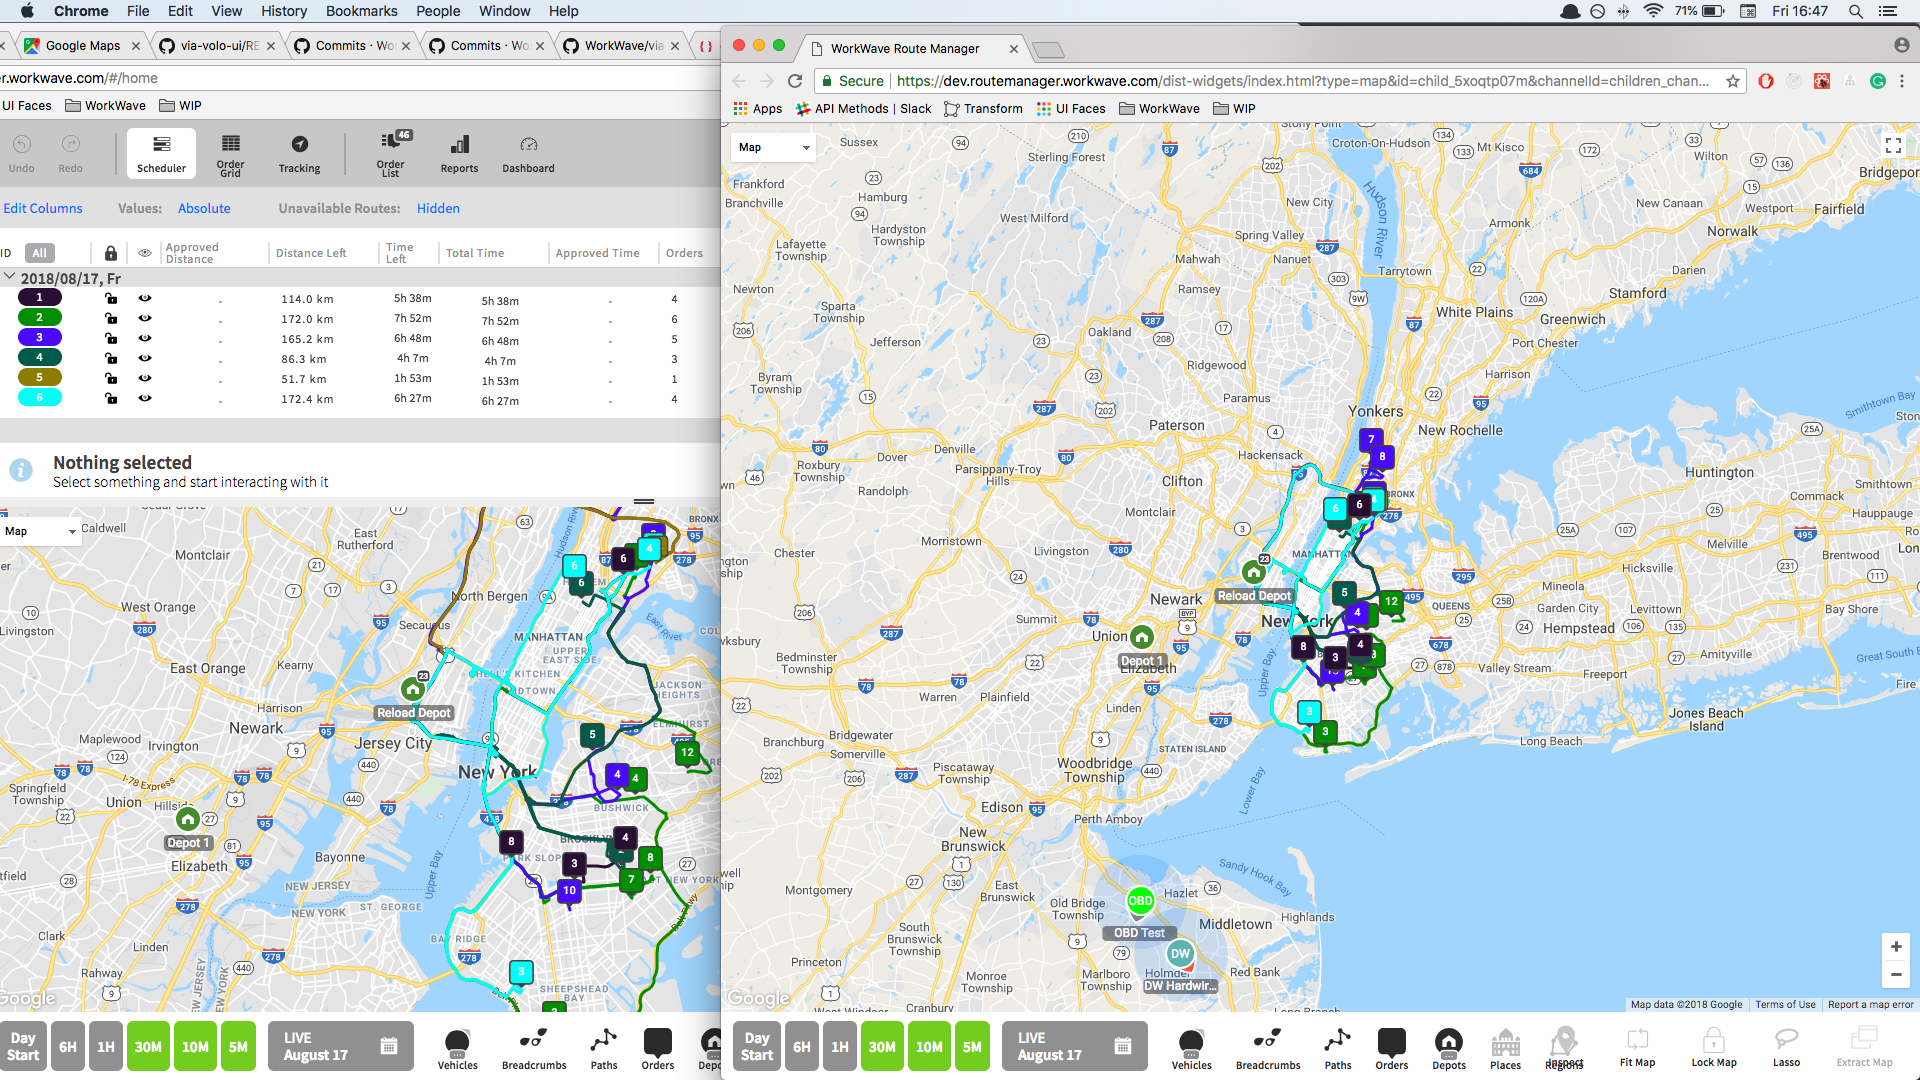
\includegraphics[width=1\columnwidth]{rm-stargate} 
    \caption{WorkWave Route Manager con Google Maps in una nuova finestra attraverso Stargate}
\end{figure}
  
%**************************************************************
\section{Obiettivi}

Si farà riferimento agli obiettivi secondo le seguenti notazioni:

\begin{itemize}
    \item \textbf{O} per i requisiti obbligatori, vincolanti in quanto obiettivo primario richiesto dal committente;
    \item \textbf{D} per i requisiti desiderabili, non vincolanti o strettamente necessari, ma dal riconoscibile valore aggiunto;
    \item \textbf{F} per i requisiti facoltativi, rappresentanti valore aggiunto non strettamente competitivo.
\end{itemize}

Le sigle precedentemente indicate saranno seguite da una coppia sequenziale di numeri, identificativo del requisito. Si prevede quindi lo svolgimento dei seguenti obiettivi:

\begin{table}[H]
\small
\begin{tabular}{ |p{2cm} |p{11cm}|}
\hline
\textbf{ID} & \textbf{Descrizione} \\ \hline

\multicolumn{2}{|c|}{\textbf{Obbligatori}} \\ \hline

O01 & Supporto multi-finestra di componenti React \\ \hline
O02 & Supporto per grandi moli di dati in continuo aggiornamento, dell'ordine di alcuni MByte \\ \hline
O03 & Supporto a molteplici finestre in contemporanea, tutte sincronizzate rispetto all'applicazione padre \\ \hline
O04 & Supporto per i browser moderni Google Chrome v56 e Firefox v38 \\ \hline
O05 & Supporto a multi-sessione \\ \hline
O06 & Gestione della configurazione di \textit{Route Manager} per supportare i widget \\ \hline
O07 & Produzione della documentazione d'uso di \textit{Stargate} \\ \hline
O08 & Utilizzo del linguaggio TypeScript v3 \\ \hline

\multicolumn{2}{|c|}{\textbf{Desiderabili}} \\ \hline

D01 & Possibilità di eseguire il componente in una nuova pagina che risieda su un processo separato del sistema operativo \\ \hline
D02 & Supporto prestazionale fino ad almeno 5 tabs simultanee \\ \hline
D03 & Supporto librerie JavaScript non React, ad esempio Angular 2 \\ \hline

\multicolumn{2}{|c|}{\textbf{Facoltativi}} \\ \hline

O04 & Supporto per i browsers Internet Explorer v11 e Edge v12 \\ \hline

\end{tabular}
\caption{Tabella degli obiettivi}
\end{table}

%**************************************************************
\section{Pianificazione}

In accordo col tutor aziendale Matteo Ronchi, l'attività dello stage è stata suddivisa nelle seguenti fasi:

\begin{itemize}
    \item \textbf{Fase 1}: Analisi dello stato dell'arte per la comunicazione cross-page in JavaScript;
    \item \textbf{Fase 2}: Realizzazione Proof of Concept in React e Redux;
    \item \textbf{Fase 3}: Implementazione dell'integrazione del widget Google Map in \textit{Route Manager} ed evoluzione della libreria;
    \item \textbf{Fase 4}: Validazione e stesura documentazione.
\end{itemize}

Non vi è stata invece necessità di un periodo iniziale di formazione sulle tecnologie TypeScript, React e Redux io quanto già in mio possesso. Mi sono anche trovato subito a mio agio con i processi di sviluppo aziendali, già incontrati da me in altre occasioni. \\

Essendo inoltre un'attività di Ricerca e Sviluppo, vi è stata una continua interazione col tutor aziendale per la definizione dei successivi step, ma a monte è stata pianificata un'ipotetica suddivisione delle ore nel seguente modo: \\

\begin{table}[H]
\small
\begin{tabular}{ |p{2cm} |p{10cm}|}
\hline
\textbf{Ore} & \textbf{Descrizione dell'attività} \\ \hline

40 & Analisi dello stato dell'arte tecnologico \\ \hline
80 & Realizzazione Proof of Concept in React e Redux \\ \hline
32 & Progettazione architetturale \\ \hline
104 & Integrazione in \textit{Route Manager} del widget Google Maps \\ \hline
24 & Gestione configurazione per supportare widget \\ \hline
16 & Validazione e Collaudo \\ \hline
8 & Refactoring prima del rilascio in produzione \\ \hline
8 & Stesura documentazione \\ \hline

\multicolumn{2}{|c|}{\textbf{Totale: 312 ore}} \\ \hline

\end{tabular}
\caption{Tabella della suddivisione delle ore}
\end{table}

\begin{figure}[H] 
    \centering 
    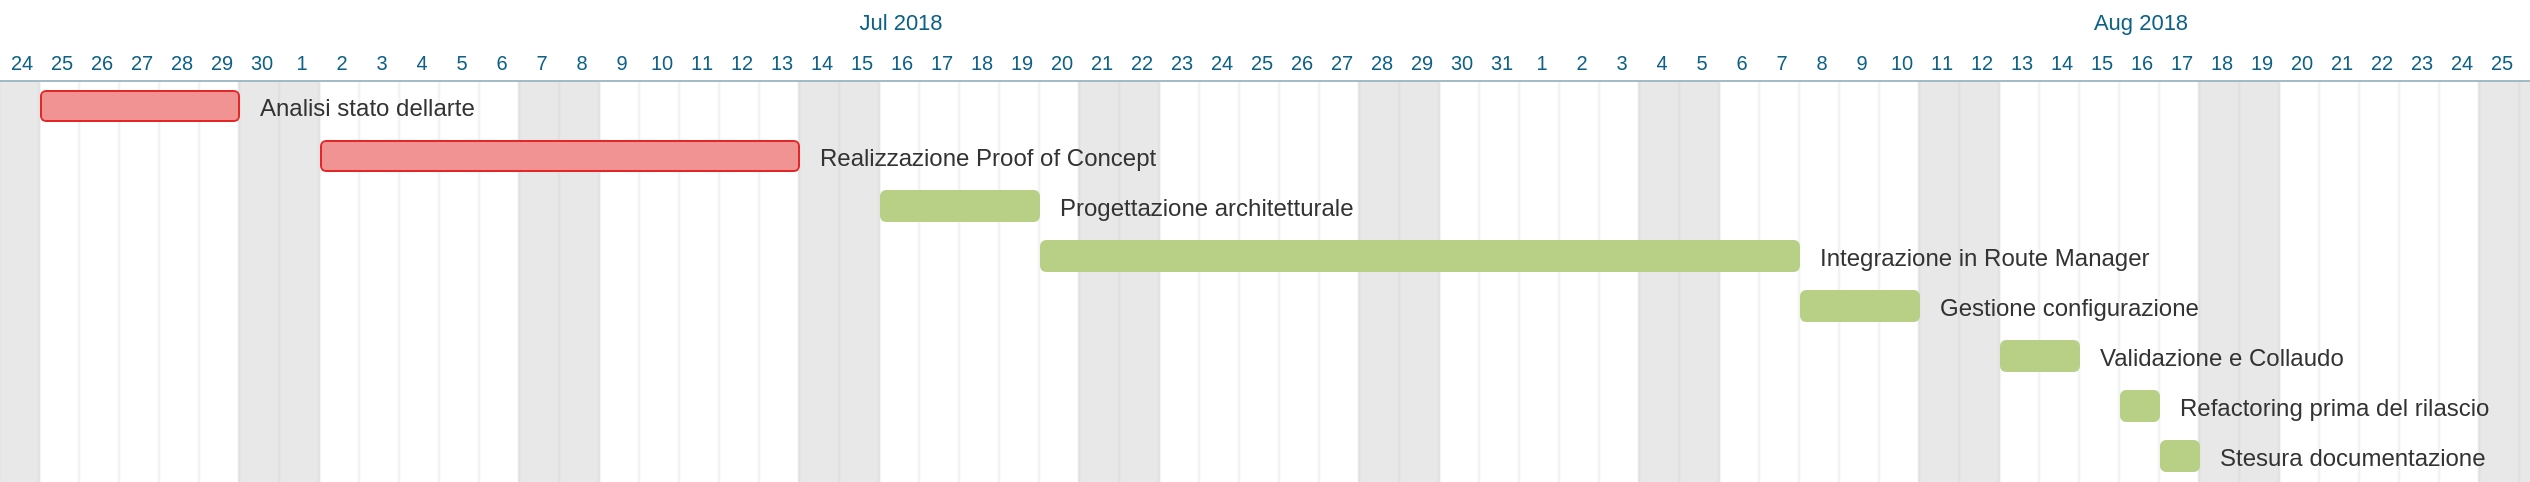
\includegraphics[width=1\columnwidth]{gantt} 
    \caption{Diagramma Gantt della pianificazione}
\end{figure}

%**************************************************************
\section{Analisi preventiva dei rischi}

Durante la fase di analisi iniziale sono stati individuati alcuni possibili rischi a cui si potrà andare incontro.
Si è quindi proceduto a elaborare delle possibili soluzioni per far fronte a tali rischi.\\

\begin{table}[H]
\small
\begin{tabular}{ |p{4.5cm} |p{4.5cm} |p{3cm}|}
\hline
\textbf{Descrizione} & \textbf{Piano di emergenza} & \textbf{Rischio} \\ \hline
\textbf{Difficoltà tecnologica}: vi è il rischio che lo stato dell'arte dello sviluppo web non consenta di aprire finestra come processi separati o che non sia possibile effettuare un'efficiente comunicazione tra pagine diverse. & È importante effettuare un'attenta attività di ricerca iniziale, al fine di comprendere lo stato dell'arte per quanto riguarda la comunicazione cross-page in applicazioni web. \newline In caso di difficoltà nella ricerca della soluzione tecnica ideale, si adotterà quella con miglior compromesso di affidabilità-performance tra quelle disponibili. & Occorrenza: Alta \newline Pericolosità: Alta \\ \hline

\textbf{Difficoltà di integrazione}: vi è il rischio che non sia possibile integrare le tecnologie adottate nel contesto dell'applicazione \textit{Route Manager}, in quanto è già in sviluppo da oltre un anno e non progettata in partenza per essere multi-finestra. & In caso di verifica del rischio, si analizzerà il problema col tutor Matteo Ronchi per trovare la miglior soluzione da adottare in \textit{Stargate} oppure in \textit{Route Manager} & Occorrenza: Alta \newline Pericolosità: Alta \\ \hline
\end{tabular}
\caption{Tabella dell'analisi dei rischi}
\end{table}

\section{Aspettative aziendali}

L'azienda WorkWave spera grazie allo stage di poter implementare una funzionalità fortemente desiderata nei loro prodotti software, in particolare in \textit{Route Manager}, con la possibilità di mostrare su pagine diverse qualsiasi componente dell'interfaccia. Ciò apre difatti le porte per una serie di possibili nuove interazioni da parte dell'utente. \\

La prima immediata conseguenza è il poter mostrare la mappa Google Maps su un monitor esterno ed in full-screen, estremamente utile sia durante i meeting che negli uffici del clienti del \textit{Route Manager} per tenere sotto costante monitoraggio le rotte ed i veicoli. Il tutto mantenendo contemporaneamente aperta l'applicazione principale su un'altra pagina, ove poter fare le modifiche alle pianificazioni ed altre attività. \\

Un ulteriore caso d'uso è la possibilità di aprire qualsiasi componente in una nuova pagina, permettendo agli utenti di customizzare i propri flussi di lavoro in modo da tenere sempre aperte alcuni widget durante la navigazione all'interno dell'applicazione. \\

Infine per l'azienda è anche un'opportunità di conoscere il tirocinante ed instaurare una conoscenza che potrà poi essere portata avanti tramite apertura di una posizione lavorativa. 

\section{Aspettative personali}

Ho intrapreso questo stage con l'obiettivo primario di venire in contatto con un ambiente di lavoro focalizzato sul team e sulla qualità dei loro prodotti. Ritengo difatti fondamentale apprendere non solo conoscenze tecniche, ma anche skill sociali e sul modo di lavorare. Grazie a WorkWave ho avuto quindi l'opportunità di conoscere cosa significhi lavorare in squadra, fare \gls{Pair Programming} per pensare insieme alla risoluzione di un problema e condividere le esperienze nella realizzazione ed evoluzione di un prodotto proprio dell'azienda. \\

È altresì importante professionalmente il contatto con i processi lavorativi di un'azienda che opera a livello world-wide, ma cercando al coltempo di mantenersi agile ed efficiente. È stata difatti concordata la possibilità di partecipare agli \gls{standup} e sono stati spiegati gli strumenti di pianificazione e comunicazione interni. \\

Ritengo inoltre indispensabile confrontarmi con colleghi molto più esperti e con maggiore esperienza, in particolare il tutor Matteo Ronchi, che ha condiviso pazientemente le ragioni dietro decisioni architetturale apprese grazie alla sua esperienza in progetti passati. 
Infine è molto istruttivo rendersi conto del livello delle conoscenze richieste per realizzare ed evolvere un prodotto complesso come \textit{Route Manager}, sia a livello di Design/User Experience che di sviluppo tecnico.
